\documentclass[12pt, twoside]{article}
\usepackage[letterpaper, margin=1in, headsep=0.2in]{geometry}
\setlength{\headheight}{0.6in}
%\usepackage[english]{babel}
\usepackage[utf8]{inputenc}
\usepackage{microtype}
\usepackage{amsmath}
\usepackage{amssymb}
%\usepackage{amsfonts}
\usepackage{siunitx} %units in math. eg 20\milli\meter
\usepackage{yhmath} % for arcs, overparenth command
\usepackage{tikz} %graphics
\usetikzlibrary{quotes, angles}
\usepackage{graphicx} %consider setting \graphicspath{{images/}}
\usepackage{parskip} %no paragraph indent
\usepackage{enumitem}
\usepackage{multicol}
\usepackage{venndiagram}

\usepackage{fancyhdr}
\pagestyle{fancy}
\fancyhf{}
\renewcommand{\headrulewidth}{0pt} % disable the underline of the header
\raggedbottom
\hfuzz=2mm %suppresses overfull box warnings

\usepackage{hyperref}

\fancyhead[LE]{\thepage}
\fancyhead[RO]{\thepage \\ Name: \hspace{4cm} \,\\}
\fancyhead[LO]{BECA / Dr. Huson / Geometry\\*  Unit 6: Analytic geometry\\* 9 January 2023}

\begin{document}

\subsubsection*{6.10 Quiz corrections: Slope-intercept form of linear equations \hfill 8.F.A.3}
\begin{enumerate}

\item Two lines are shown in the graph below.
\begin{multicols}{2}
    \begin{enumerate}[itemsep=0.5cm]
      \item Write down their equations in slope-intercept form. \vspace{1.5cm}
      \item Write down their intersection as an ordered pair. \vspace{0.7cm}
      \item Show that the lines are not perpendicular by taking the product of their slopes. \vspace{1cm}
      \end{enumerate}
    \begin{flushright}
    \begin{tikzpicture}[scale=0.8]
      \draw [help lines] (-1,-2) grid (6,5);
      \draw [thick, ->] (-1.2,0) -- (6.4,0) node [below right] {$x$};
      \draw [thick, ->] (0,-2.2)--(0,5.4) node [right] {$y$};
      \draw [fill] (0,5) circle [radius=0.05] node[below left] {$A(0,5)$};
      \draw [fill] (0,-2) circle [radius=0.05] node[below right] {$B(0,-2)$};
      \draw [fill] (3,1) circle [radius=0.05] node[right] {$C(3,1)$};
      \draw [<->, thick, domain=-0.4:5.2] plot (\x,-1.333*\x+5);
      \draw [<->, thick, domain=-0.4:5.2] plot (\x,\x-2);
    \end{tikzpicture}
    \end{flushright}
  \end{multicols} \vspace{2cm}

\subsubsection*{The midpoint formula}
\item Write down the midpoint formula. \vspace{1cm}

\item In the diagram below, $\overline{AB}$ has endpoints with coordinates $A(2,1)$ and $B(8,4)$. Find the coordinates of the midpoint $M$ of $\overline{AB}$. Mark and label it on the graph.
\begin{flushright}
  \begin{tikzpicture}[scale=.6]
    \draw [help lines] (-3,-2) grid (9,7);
    \draw [thick, <->] (-3.4,0) -- (9.4,0) node [below right] {$x$};
    \draw [thick, <->] (0,-2.4)--(0,7.4) node [left] {$y$};
    \draw [thick] (2,1)--(8,4);
    \draw [fill] (2,1) circle [radius=0.1] node[above left] {$A$};
    \draw [fill] (8,4) circle [radius=0.1] node[below right] {$B$};
  \end{tikzpicture}
\end{flushright}

\newpage

\subsubsection*{The distance formula}
\item Write down the distance formula. \vspace{1cm}

\item What is the length of $\overline{PQ}$ if $P(2,1)$ and $Q(10,7)$? \vspace{4cm}

\item Graph and label $\triangle ABC$. Calculate the lengths of its sides. $A(0,0)$, $B(12,5)$, $C(12,0)$.
\begin{flushleft}
    \begin{tikzpicture}[scale=.635]
    \draw [help lines] (0,0) grid (13,8);
    \draw [thick, ->] (0,0) -- (13.4,0) node [below right] {$x$};
    \draw [thick, ->] (0,0)--(0,8.4) node [right] {$y$};
    \foreach \x in {1,...,13}
    \draw[shift={(\x,0)}] (0pt,-3pt)--(0pt,3pt) node[below=5pt] {$\x$};
    \foreach \y in {1,...,8}
    \draw[shift={(0,\y)}] (-3pt,0pt)--(3pt,0pt) node[left=5pt] {$\y$};
    \end{tikzpicture}
\end{flushleft} \vspace{3cm}

\item Write the linear equation $4x+2y=10$ in the form $y=mx+b$. \vspace{4cm}

\end{enumerate}
\end{document}